\documentclass{article}
\usepackage[italicdiff]{physics}
\usepackage{tikz}

\title{On measuring heights}
\author{Alden Bradford}

\begin{document}

\maketitle

\begin{quote}
Some engineers are trying to measure the height of a flagpole. They only have a measuring tape, and they have not been able to slide the tape up the pole. A mathematician asks what they are doing, and they explain.

``The solution is easy," he says. He pulls the pole out of the ground, lays it down, and measures it.

After he leaves, one of the engineers says, ``That is so typical! We tell a mathematician that we need to know the height -- and he gives us the length!"

\hfill -G. Patrick Vennebush, ``Math Jokes 4 Mathy Folks", p.72
\end{quote}

Suppose you want to know how tall a flagpole is, and you only have an inclinometer and a rope of a known length. Most flagpoles are installed perpendicular to the ground, so we can figure this out using a bit of trigonometry. Consider the following figure.

\begin{figure}[h!]
\centering
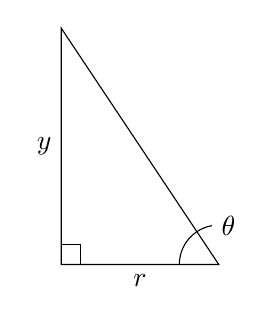
\begin{tikzpicture}
	\draw (0, 0) -- node[anchor=north] {$r$} (2, 0) -- (0, 3) -- node[anchor=east] {$y$} cycle;
	\draw (0.25, 0) -- (0.25, 0.25) -- (0, 0.25);
	\draw (1.5,0) arc (180:100:0.5) node[anchor=west] {$\theta$};
\end{tikzpicture}
\end{figure}

You probably know from trigonometry that these quantities are related by the tangent function: $y = r \tan \theta$. If the flagpole is represented by the vertical line, you could lay out your rope from the base of the flagpole and represent it by the horizontal line in the figure. Then get down on the ground, and with your eye at the end of the rope, sight an angle $\theta$ up to the top of the flagpole. then just compute $\tan\theta$ times the length of the rope, and you have the height of the flagpole.

Of course, it's pretty uncomfortable to get on the ground. It would be better to measure from standing up. That's easy to do, just measure the height $k$ up to your eyeball and draw the figure as so:
\begin{figure}[h!]
\centering
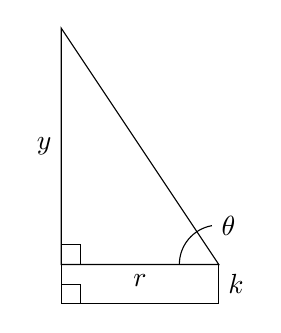
\begin{tikzpicture}
	\draw (0, 0) -- node[anchor=north] {$r$} (2, 0) -- (0, 3) -- node[anchor=east] {$y$} cycle;
	\draw (0.25, 0) -- (0.25, 0.25) -- (0, 0.25);
	\draw (1.5,0) arc (180:100:0.5) node[anchor=west] {$\theta$};
	\draw (0, 0) -- (0, -0.5) -- (2, -0.5) -- node[anchor=west] {$k$} (2, 0);
	\draw (0, -0.25) -- (0.25, -0.25) -- (0.25, -0.5);
\end{tikzpicture}
\end{figure}

Then the height of the flagpole would be simply $h = y+k$. You just have to add your eye-height to the value computed using the rope, $h=r\tan\theta+k$. Now you don't have to put your face to the ground.

What if you wanted to measure the height of a mountain? You can't very well put one end of the rope underneath the summit without digging a serious tunnel. Luckily, there is a better way. This method has been used since ancient times by pacific islanders. All you need is to lay your rope directly pointed towards the top of the mountain on level ground, not necessarily touching the mountain at all. Stand at each end of the rope and sight an angle to the summit. This gives a picture like so:

\begin{figure}[h!]
\centering
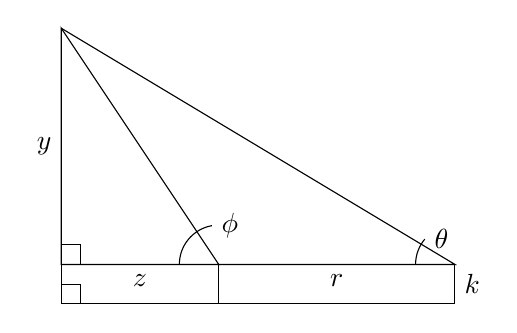
\begin{tikzpicture}
	\draw (0, 0) -- node[anchor=north] {$z$} (2, 0) -- (0, 3) -- node[anchor=east] {$y$} cycle;
	\draw (0.25, 0) -- (0.25, 0.25) -- (0, 0.25);
	\draw (1.5,0) arc (180:100:0.5) node[anchor=west] {$\phi$};
	\draw (0, 0) -- (0, -0.5) -- (2, -0.5) -- (2, 0);
	\draw (0, -0.25) -- (0.25, -0.25) -- (0.25, -0.5);
	\draw (2, 0) -- node[anchor=north] {$r$} (5, 0) -- (0, 3);
	\draw (4.5,0) arc (180:140:0.5) node[anchor=west] {$\theta$};
	\draw (2, -0.5) -- (5, -0.5) -- node[anchor=west] {$k$} (5, 0);
\end{tikzpicture}
\end{figure}

Once again your rope is along the line marked $r$ and the height to be determined is $h=y+k$. $z$ represents the distance from the nearer end of the rope to the point directly below the summit. We can apply the trigonometry rule twice here to get two equations:
\begin{align*}
y &= z \tan \phi\\
y &= (z+r) \tan \theta
\end{align*}
We could rearrange the first to say $z = y \cot \phi$, and substitute into the second. Without too much algebra you can show this means
\[
h = \frac{r}{\cot \theta -\cot \phi}+k.
\]

So, to compute the height of a far-off thing, you can stand at either end of a rope, measure the angle to the top from eye level, and apply this formula.

\end{document}